%%%%%%%%%%%%%%%%%%%%%%%%%%%%%%%%%%%%%%%%%%%%%%%%%%%%%%%%%%
%
% Vzor pro sazbu kvalifikační práce
%
% Západočeská univerzita v Plzni
% Fakulta aplikovaných věd
% Katedra informatiky a výpočetní techniky
%
% Petr Lobaz, lobaz@kiv.zcu.cz, 2016/03/14
%
%%%%%%%%%%%%%%%%%%%%%%%%%%%%%%%%%%%%%%%%%%%%%%%%%%%%%%%%%%

% Možné jazyky práce: czech, english
% Možné typy práce: BP (bakalářská), DP (diplomová)
\documentclass[english,BP]{thesiskiv}

% Definujte údaje pro vstupní strany
%
% Jméno a příjmení; kvůli textu prohlášení určete, 
% zda jde o mužské, nebo ženské jméno.
\author{Roman Kalivoda}
\declarationmale

%alternativa: 
%\declarationfemale

% Název práce
\title{Extension of neural network architecture}

% 
% Texty abstraktů (anglicky, česky)
%
\abstracttexten{The text of the abstract (in English). It contains the English translation of the thesis title and a short description of the thesis.}

\abstracttextcz{Text abstraktu (česky). Obsahuje krátkou anotaci (cca 10 řádek) v češtině. Budete ji potřebovat i při vyplňování údajů o bakalářské práci ve STAGu. Český i anglický abstrakt by měly být na stejné stránce a měly by si obsahem co možná nejvíce odpovídat (samozřejmě není možný doslovný překlad!).
}

% Na titulní stranu a do textu prohlášení se automaticky vkládá 
% aktuální rok, resp. datum. Můžete je změnit:
%\titlepageyear{2016}
%\declarationdate{1. března 2016}

% Ve zvláštních případech je možné ovlivnit i ostatní texty:
%
%\university{Západočeská univerzita v Plzni}
%\faculty{Fakulta aplikovaných věd}
%\department{Katedra informatiky a výpočetní techniky}
%\subject{Bakalářská práce}
%\titlepagetown{Plzeň}
%\declarationtown{Plzni}

%%%%%%%%%%%%%%%%%%%%%%%%%%%%%%%%%%%%%%%%%%%%%%%%%%%%%%%%%%
%
% DODATEČNÉ BALÍČKY PRO SAZBU
% Jejich užívání či neužívání záleží na libovůli autora 
% práce
%
%%%%%%%%%%%%%%%%%%%%%%%%%%%%%%%%%%%%%%%%%%%%%%%%%%%%%%%%%%
% for inserting landscape oriented pages
\usepackage{pdflscape}

% Enables long table to be split
%\usepackage{longtable}

% More adjustable table environment
\usepackage{tabularx}

% Professional looking tables
\usepackage{booktabs}

% Improves justification
\usepackage{microtype}

% balík pro import dílčích .tex souborů do hlavního
%\usepackage{import}

\usepackage{csquotes}

% Zařadit literaturu do obsahu
\usepackage[nottoc,notlot,notlof]{tocbibind}

% Umožňuje vkládání obrázků
\usepackage[pdftex]{graphicx}

% SVG image support
\usepackage{svg}

% To rotate the appendices
\usepackage{rotating}

\graphicspath{ {./images/} }

% Odkazy v PDF jsou aktivní; navíc se automaticky vkládá
% balíček 'url', který umožňuje např. dělení slov
% uvnitř URL
\usepackage[pdftex]{hyperref}
\hypersetup{colorlinks=true,
  unicode=true,
  linkcolor=black,
  citecolor=black,
  urlcolor=black,
  bookmarksopen=true}

% Při používání citačního stylu csplainnatkiv
% (odvozen z csplainnat, http://repo.or.cz/w/csplainnat.git)
% lze snadno modifikovat vzhled citací v textu
\usepackage[backend=biber, style=ACM-Reference-Format]{biblatex}

\addbibresource{references.bib}
%\usepackage[numbers,sort&compress]{natbib}

%%%%%%%%%%%%%%%%%%%%%%%%%%%%%%%%%%%%%%%%%%%%%%%%%%%%%%%%%%
%
% VLASTNÍ TEXT PRÁCE
%
%%%%%%%%%%%%%%%%%%%%%%%%%%%%%%%%%%%%%%%%%%%%%%%%%%%%%%%%%%
\begin{document}
%
\maketitle
\tableofcontents

\chapter{Introduction}
% V souboru \texttt{literatura.bib} jsou uvedeny příklady, jak citovat knihu \cite{KnuthAOCP2}, článek v časopisu \cite{Hoare1961}, webovou stránku \cite{Graphics2D}.
A neural network is a set or population of specialized cells (neurons) that are interconnected by synapses. In biology, neural network forms the structure of a neural system in animals. The interconnection pattern, size and spatial organization of the population determines the architecture and specialization of the network. The network specializes to carry out a specific function when it is activated. These specialized networks then tie to one another to develop larger systems (e.g. animal brain). These natural phenomena inspired computer scientists to design a set of algorithms that models some aspects of the animal brain. 

Artificial (analogue) neural networks (ANNs) were initially inspired by biological neural systems but many concepts were simplified or modified to conform to their practical applications. On the other hand, the spiking neural networks (SNNs) were mostly meant to simulate their biological models as closely as possible and thus improve our understanding of how real biological networks achieve their cognitive abilities with incredibly low energy consumption. Although the differences between those approaches still last, some aspects of the two approaches are getting more interconnected as the research advances and one approach can exploit the other. Nowadays, deep ANNs achieve satisfying accuracy in many complex tasks, although with extensive requirements on computation power. Because of that, new goals for the improvement of their efficiency are being set. That is where deep SNNs appear to be an interesting topic of research because of better power efficiency \cite{caoSpikingDeepConvolutional2015, tavanaeiDeepLearningSpiking2019}, although the applications generally do not accomplish the same accuracy yet. Apart from the applications in which ANNs are used, spiking networks open up new fields of utilization. In the following sections, I will briefly summarize the differences between the two classes of neural networks and then focus on the current state of the research in the area of the spiking networks.

\section{Artificial neural networks}
Artificial neural networks are built of idealised units which compute output values from their weighted input values and continuous nonlinear activating functions \cite{tavanaeiDeepLearningSpiking2019}. The units interact with each other by propagating its continuous output. These units can be connected into distinct layers. If there is more than one hidden layer (hidden layer is the layer which takes input from the previous layer and outputs own results to another layer, that means it is neither input layer, nor output layer), the network is recognized as a deep network. In deep networks, each layer works with a set of features received from the output of the previous layer. This feature hierarchy enables deep networks to operate accurately on large data sets with plenty of parameters. Advances in the hardware computation power made possible to use very deep networks for various artificial intelligence tasks. However, the (still quite) great computation costs of these networks prevent them from applications in embedded and power-constrained environments. \par
To become functional, the resulting neural network needs to be learned. Learning neural network means adjusting its connection weights and other parameters to optimise the accuracy of the results. There exist two major approaches to learning of a neural network, supervised learning and unsupervised learning. \par

\subsection{Supervised learning in artificial neural networks}
A prerequisite for the supervised learning method is a labelled data set. Supervised learning is useful for classification or regression tasks when we need to find a set of significant relationships or structure in the input data, that means we need to approximate a regression function. The functionality of the method is dependent on the complexity of the function which is being learned. Higher complexity is needed to learn the full structure of the data, but there is a threat of over-fitting the model, that means the model will be too complex and will fail on general data. In the neural network, supervised learning is achieved with the error backpropagation algorithm. The algorithm learns the network on the learning data set and finds the difference between the computed and desired output. Then the synaptic weights are adjusted to minimise the difference \cite{sathyaComparisonSupervisedUnsupervised2013}.

\subsection{Unsupervised learning in artificial neural networks}
Unsupervised learning means that the data set is missing labels and the model attempts to find some structure in the underlying data set. Common use-cases for unsupervised learning are exploratory analysis and dimensional reduction. Exploratory analysis can be used to get an initial overview in situations where it is difficult or impossible for people to find trends in the data. Typical applications for unsupervised learning methods are data clustering or visualisation. Another example of unsupervised learning is generative adversarial networks (GANs). GANs is an architecture that uses two neural networks to generate new synthetic data with a structure similar to real data \cite{goodfellowGenerativeAdversarialNets2014}.

\section{Spiking neural networks}
Although the basic principle of artificial neural networks is inspired by biological neural networks, the processes in the biological networks differ from the processes in ANNs. The spiking neural networks are built upon knowledge retrieved from observations of the biological neural networks. The basic idea behind SNN is that the network consists of the spiking neurons which have a different characteristic than artificial neurons. Each spiking neuron has a specified threshold value and membrane potential. Note that the resting membrane potential of the real biological neuron is typically negative, but for mathematical simplification, it is convenient to assume in the spiking neuron models, that the resting membrane potential is zero and thus the current membrane potential is the sum of postsynaptic potentials \cite{maassNetworksSpikingNeurons1997}. The postsynaptic potential is a result of action potential (spike) generated by previous neurons which are connected to the observed neuron. The postsynaptic potential can be either excitatory or inhibitory. The excitatory postsynaptic potential (EPSP) increments (depolarise) the membrane potential and the inhibitory postsynaptic potential decrements (hyper-polarise) the membrane potential. When the membrane potential reaches the threshold value of the neuron, a spike (a sudden increase of voltage) is generated. It can also be said that the neuron fired. Depending on the level of detail, various models of spiking neuron exist. Popular spiking neuron models are the leaky integrate-and-fire model (LIF), the Izhikevich neuron model or spike response model \cite{tavanaeiDeepLearningSpiking2019}. \par
Besides the biological perspective on spiking neural networks, there also exists a more technical point of view used in neuromorphic engineering. In this perspective, the spikes are more often called events. This term originates from the address event representation protocol \cite{pazTestInfrastructureAddressEventRepresentation2005, boahenPointtopointConnectivity00} which is used to connect event-based neuromorphic peripherals. With this point of view, the emphasis on the biological plausibility of the model and level of detail of the neurons is sidelined to allow more pragmatic ways to use the networks in such neuromorphic applications. The combination of the spiking neural networks with event-based sensors is especially useful because it enables both parts to utilise its full potential in terms of power efficiency \cite{pfeifferDeepLearningSpiking2018}.

\section{Deep spiking neural networks}
Similar to ANNs, if the spiking neural network consists of multiple layers and at least one of them is hidden, the network is called deep. Deep neural networks, both spiking and non-spiking are more capable. The interconnected neurons transfer information between themselves by firing trains of spikes (spike trains). Strictly speaking, the information is coded in the number of spikes and their frequencies, rather than the amplitude characteristic of a single spike. That means the communication in the network is discrete in time in contrast to ANN where the communication is based on continuous activation functions. This makes the spiking neural networks interesting to research because SNNs can be used to create more efficient low-energy consuming neural networks. Also, SNNs can be implemented on special dedicated hardware, which even more improves energy efficiency. Another advantage of the spiking deep networks is that the approximation of the final layer output can be retrieved at the time of recording first input spikes and the approximation improves over time \cite{pfeifferDeepLearningSpiking2018}.
Deep spiking neural networks have theoretically the same representational power as deep ANNs with lower energy requirements. But there is a problem with achieving the same results as with ANNs because optimal solutions for supervised learning of the SNNs do not exist yet. The gradient-based optimisation methods used in the artificial neural networks require the activation function to be differentiable \cite{tavanaeiDeepLearningSpiking2019}. The spike trains generated in spiking neurons can be formally represented by sums of delta functions which do not have derivatives. To overcome this problem, multiple approaches were proposed, but the research of the learning methods for the SNNs is still at its beginning \cite{tavanaeiDeepLearningSpiking2019}. 

\section{State of the art}
Recently there appeared many novel theories and experiments on the topic of the deep spiking neural networks and new approaches to learning such networks. As stated above, traditional methods for deep learning can be hardly used because of the distinct characteristics of the two models. One of the approaches to overcome this issue is using some sort of approximate derivatives or other substitutes, although this may reduce bio-plausibility of the model. \cite{leeTrainingDeepSpiking2016} proposed a spiking network backpropagation rule with low-pass filtering to handle discontinuity at the time of the spike. This method demonstrates state-of-the-art results for deep SNNs.\par
The more bio-plausible approach is using local learning rules such as spike-timing-dependent plasticity (STDP). STDP adjusts the synaptic weights between presynaptic and postsynaptic neuron according to the relative difference of their spike times. If presynaptic neuron fires relatively briefly before the postsynaptic neuron, their synaptic weight is increased. The weight is decreased in the opposite case, that is in the case when presynaptic neuron spikes briefly after the postsynaptic neuron. Local learning rules can be used with unsupervised learning \cite{tavanaeiDeepLearningSpiking2019}, but with supervised learning, there is once again missing a plausible backpropagation method. This problem can be covered for example by introducing recurrent connections to propagate the error signal. The use of local learning rules is also interesting for efficient implementations on dedicated hardware, such as SpiNNaker\cite{furberSpiNNakerProject14} or BrainScales. At present, the efficiency of the networks which use this method falls behind in terms of accuracy. \par
Another approach is to create a conversion between ANN and SNN. For the conversion, a conventional deep network is trained using backpropagation and other methods available in ANNs. Then the already trained network is transformed into its spiking variant. This is done by mapping the analogue neurons onto spiking ones (the mapping can be both one-to-one and one-to-many) and adjusting the weights and parameters of the spiking neurons according to the trained analogue network. The conversion approach was first proposed in \cite{perez-carrascoMappingFrameDriven13}. This approach can be used to enhance the performance of hardware implementations of deep neural networks. An advantage of this approach is that the best, state-of-the-art deep networks can be transformed into SNNs without previous modifications and the efficiency of the final SNN is approaching the efficiency of the original network. However not every ANN can be converted, because features or methods which are common in analogue networks might not have its spiking equivalents. \cite{rueckauerConversionContinuousValuedDeep2017} introduced additional techniques to convert more general class of ANNs by implementing features such as soft-max, batch normalisation or max-pooling (using a maximum filter for spatial reduction of the input feature set), which were previously not available in the spiking networks. The resulting accuracy of experiments which used the conversion approach is very promising \cite{tavanaeiDeepLearningSpiking2019, pfeifferDeepLearningSpiking2018}. One of the disadvantages of the conversion is that the most often used technique uses rate codes which are quite inefficient. Rate-coding means that the activation values of the original analogue deep network are translated into firing rates of the spiking neurons, so multiple spikes are necessary to stand for a single activation value. To overcome this, alternative spike codes are needed to be developed. \cite{zambranoFastEfficientAsynchronous2016} proposes one such coding, which maintains the accuracy of the original artificial network while reducing the total count of spikes needed in comparison to other conversion methods. \par
There exists a modified hybrid approach known as \textit{constrain-then-train}. Instead of starting with conventional learning of the ANN, additional constraints needed for spiking networks (or target neuromorphic platform) are applied on the initial network before it is trained. Then, the learned parameters of such constrained ANN can be used directly during the mapping onto SNN without further re-scaling \cite{pfeifferDeepLearningSpiking2018}. The retrieved parameters are particular for just one setting of the spiking neuron model, so the network needs to be retrained if these parameters should change. The final network has an advantage that it adapts better to the target environment than generally converted networks. \par
Above four approaches to supervised learning of the spiking neural networks are briefly described. The spike-based learning and local learning methods have a common need for improvement of the accuracy to match the results retrieved by the other two methods, but they offer other notable features such as potentially better energy efficiency and the ability to exploit additional features of the neuromorphic hardware (e.g. precise timing). Also, inferior performance efficiency is being improved by recent works. On the other hand, the conversion techniques are comparable to its artificial network original models, but due to the used coding, its energy efficiency is deteriorated.

\subsection{Binary deep neural networks}
Binary deep neural networks (BNNs) are an alternative to spiking neural networks in terms of energy efficiency. BNNs are deep neural networks that use binary activation values and/or binary-valued weights \cite{simonsReviewBinarized19}. The state-of-the-art binary neural networks achieve slightly degraded accuracy in comparison with non-binary full precision networks, but with reduced memory requirements and less power consumption \cite{courbariauxBinarizedNeural16}. This is more evident if both activation values and weights are binary as more complex arithmetic operations can be replaced with simpler bitwise operations \cite{kimBitwiseNeural16}. With binary activations, BNNs can also directly use spikes from event-based hardware \cite{linAccurateBinary17}. Compared to spiking networks, the information is still propagated synchronously and does not allow the fast propagation of most salient features \cite{pfeifferDeepLearningSpiking2018}.

\subsection{Comparison}
To compare the individual works, common classification benchmarks are used usually, although \cite{pfeifferDeepLearningSpiking2018} points out that these benchmarks might not be appropriate for evaluation of spiking networks and should be taken as a proof of concept. The most used benchmark for demonstrating the performance of the spiking network is the MNIST data set of handwritten digits. Table \ref{tab:MNIST_benchmark} compares some of the reported classification accuracies on the MNIST data set.

\begin{table}[htbp]
    \centering
    \begin{tabularx}{\linewidth}{|>{\raggedright\arraybackslash}X|c|c|}
    \hline
        description & type & accuracy (\%) \\
        \hline
        \hline
        Rate-based conversion of 7-layer CNN with max-pooling \cite{rueckauerConversionContinuousValuedDeep2017} & SNN & 99.44 \\
        \hline
        Converted SNN with pulsed Sigma-Delta coding scheme \cite{zambranoFastEfficientAsynchronous2016} & SNN & 99.14 \\
        \hline
        Converted Lenet-5 with TTFS temporal coding \cite{rueckauerConversionAnalogSpiking2018} & SNN & 98.57 \\
        \hline
        Spiking CNN with low-pass backpropagation rule \cite{leeTrainingDeepSpiking2016} & SNN & 99.31 \\
        \hline
        Branching \& Merging CNN with Homogenous filter capsules \cite{kalganovaBranchingMerging20} & ANN & 99.79 \\
        \hline
        Multi-column deep neural network \cite{cireganMulticolumnDeep12} & ANN & 99.77 \\
    \hline
    \end{tabularx}
    \caption{Comparison of selected deep neural networks.}
    \label{tab:MNIST_benchmark}
\end{table}

\chapter{Comparison of available simulation platforms}
Currently, there exist numerous platforms for simulation of biological neural networks. The first objective is to analyse those platforms from the perspective of their capabilities and choose the most suitable of them. The main criterion is the current state of the community and user base around the platform, their ability to provide support to the users and state of the project documentation. Because many of the projects are using GitHub to host its repositories, the metrics like code frequency, contributors count, number of issues and similar indicators displayed by GitHub can help to determine this. The next criterion is whether the platform provides means to interact with both spiking neural networks and artificial neural networks. Other criteria are user-friendliness of the platform and license conditions. The Neural Simulation Tool (NEST) \cite{jordanNEST182019}, Brian \cite{stimbergBrianIntuitiveEfficient2019}, Neuron \cite{carnevaleNEURONBook06} and Nengo \cite{bekolayNengoPythonTool2014} are platforms, which were analysed more precisely. Other projects, that is Multiscale Object-Oriented Simulation Environment (MOOSE), STochastic Engine of Pathway Simulation (STEPS), Topographica, Neocortical Simulator (NCS), The Parallel Circuit SIMulator (PCSIM) and the GEneral NEural SImulation System (GENESIS) were not included out of consideration for their small community, range of supported models and/or because they are no longer actively developed. At the end of this chapter, I will also mention PyNN, simulator-independent language for building neuronal network models \cite{davisonPyNNCommonInterface2009}. PyNN works as a frontend for Neuron, NEST and Brian simulators.

\section{The Neural Simulation Tool (NEST)}

NEST is a simulator for spiking neural network models. Its development is coordinated by the NEST initiative. NEST provides approximately 50 neuron models and over 10 synapse models. Its primary focus is on the dynamics, size and structure of the network rather than on the exact morphology of individual neurons. NEST is implemented in C++ and contains a scripting interface for Python and its native simulation language interpreter (SLI). Recently, a new markup language NESTML was developed to make the creation of new neuron models easier \cite{plotnikovNESTMLModelingLanguage2016}.  NEST can be used on many computer architectures from low-end laptops to supercomputers. Project's page explicitly mentions Linux, MacOS X and IBM BlueGene as supported platforms. Windows operating system can utilize a prepared virtual machine image. The scaling of the existing model on a high-performance cluster or multi-core computer is convenient and minimal or no changes are required, which is an advantage over other simulation platforms \cite{tikidji-hamburyanSoftwareBrainNetwork2017}. NEST is used in projects like the Human Brain Project or BrainScaleS. NEST is cited in over 290 papers as the simulator which was used \cite{julichaachenresearchallianceNESTNeuralSimulation2015}.

\section{Brian}

Brian is a spiking neural network simulator written in Python. It is an equation oriented simulator, i.e. neural models are defined in its mathematical form with differential equations rather than written in programming language function. This makes the simulator very flexible. To increase the speed of simulation, Brian can run in several runtime code generation modes, for example, NumPy, Cython or generate a standalone C++ code (although some limitations apply). A Downside of the Brian software is limited support for parallel computations and total lack of support for cluster computations \cite{tikidji-hamburyanSoftwareBrainNetwork2017}. Project's page does not state any numbers of its users, but there exists a Google group \cite{Brian} with support topics, which has over 300 users. Maintainers of the project do not track any information about publications, which use Brian.

\section{Neuron}

NEURON is a simulation environment for modelling single neurons or neural networks. It specializes in empirically-based simulations. NEURON is more suitable for simulating single neuron models with more complex structure. Neuron contains a graphical user interface (GUI), which can be used to manipulate an existing model or create a new one. The GUI can be used to create both single neuron model and a network model.  Neural networks and neuron models can be described with Neuron's own interpreted language called hoc or with Python script. New modules for neuron dynamics can be developed in its native simplified language NMODL \cite{tikidji-hamburyanSoftwareBrainNetwork2017}. Neuron utilizes several methods to optimize the efficiency of its code. For example, it provides routines for tabulating values of often used equations to avoid their computation every time. It also supports optimizations for high-performance computing, such as embarrassingly parallel computation without the need to use other software. Neuron is the only simulator which can distribute computations for a single complex neuron over a cluster \cite{tikidji-hamburyanSoftwareBrainNetwork2017}. According to its web page, its user base is large with more than 1500 registered users at the forum and more than 1900 of scientific articles that reported the use of NEURON. Software installers are available for MS Windows, macOS and Linux.

\section{Nengo}

Nengo is a tool for simulating large neural models. Nengo exploits the theoretical modelling approach described by the Neural Engineering Framework. The Neural Engineering Framework proposes three principles (representation, transformation, and dynamics) for the construction of large-scale neural models which are simulator independent. Nengo decouples model creation and simulation, so multiple simulators can be used to run created models. NengoDL is one such simulator built on top of the deep learning framework TensorFlow. Nengo also provides a backend for neuromorphic hardware Intel Loihi. From version 2 onwards, Nengo is written in the Python programming language. It can be used on all major operating systems. Figure \ref{fig:nengo_ecosystem} shows a relation between the Nengo components. Nengo is published under a proprietary license which allows free manipulation with Nengo and its source code for any non-commercial purpose as long as the copyright notice is included. According to the project's webpage, Nengo was mentioned in more than 100 publications. Nengo forum has over 200 registered users of which about 40 were active last month.

\begin{figure}[ht]
    \centering
    \includesvg[width=\textwidth]{nengo_ecosystem}
    \caption{The Nengo ecosystem. Source: \url{https://www.nengo.ai/documentation/}}
    \label{fig:nengo_ecosystem}
\end{figure}

\subsection{Neural engineering framework}
The neural engineering framework (NEF) is a general method for building neural models. It can be used to solve connection weights between network components by specifying properties of the used neuron models, the values which they represent and the functions which should be computed \cite{stewartTechnicalOverviewNeural2012}. The NEF defines three principles for building large-scale neural models. These principles are called representation, transformation and dynamics. \par
The representation principle states that information is represented by a population of neurons. Neural populations represent time-varying signals through their spiking responses and a signal is perceived as a vector of real numbers of arbitrary length.  This way, neural computations can be defined by manipulating the information using conventional mathematics \cite{bekolayNengoPythonTool2014}. During the encoding process, a specific amount of current is released into a single neuron. The tuning curve of the neuron determines how likely is that neuron to spike as a function of the input signal. The encoded information is represented by the spike frequency of the population. The information can be decoded by observing these spike trains. First, the spike frequencies are filtered with exponentially decaying filter. The filtered spike trains are then multiplied with decoding weights and summed together. The accuracy of the decoded information increases with the increasing number of neurons in the population. \par
The transformation principle describes how to decode spike trains to compute transformations of signals. It provides a way to compute the connection weights between populations to represent an arbitrary function. \par
When the neurons are connected recurrently, the vectors represented by neural populations can be interpreted as state variables of the dynamical system and methods of control theory can be applied \cite{bekolayNengoPythonTool2014}.

\subsection{Semantic pointer architecture}
The semantic pointer architecture provides an approach to build cognitive models with large-scale spiking neural networks. As stated in \cite{eliasmithHowBuild13}, the semantic pointers are neural representations that carry partial semantic content and are composable into the representational structures to support complex cognition. The Semantic Pointer Architecture (SPA) uses vectors to represent concepts. The Nengo-SPA package contains the implementation of the SPA for the Nengo simulator.

\section{PyNN}
PyNN is a language for building models of neuronal networks independently of the used simulator. It provides a common API in the Python language to write the code and run it on multiple backends. PyNN API is designed to support neural networks models at a high-level of abstraction. Currently, Neuron, Brian (version 1) and NEST are supported simulators. PyNN also supports the SpiNNaker and BrainScaleS neuromorphic hardware and is partially compatible with NeuroML model description language. Figure \ref{fig:pynn_arch} shows the architecture of the PyNN interface \cite{bruderleNeuroscientificModelingMixedSignal2009}.


\section{Summary of platform comparison}
Out of available neural simulation platforms, four were chosen as the best candidates for further analysis. As a starting point for the comparison of Neuron, Brian and NEST, a previous comparative study \cite{tikidji-hamburyanSoftwareBrainNetwork2017} was used. Each of the platforms has some sort of forum or mailing list for communication of its users. Statistics retrieved from these pages were used to compare the number of users of the platform. Other statistics were retrieved from the GitHub sites of the projects as an indicator of the activity of the projects in the last years. The collected statistics are shown in Table \ref{tab:comparison} below. The Neuron simulator has by far the largest community on its user forum and is cited by other researchers most often. This is probably because the Neuron simulator is developed for the longest time. On the other hand, The NEST simulator has almost three times more contributors to its source code than any other platform. Nengo is the only simulator which offers utilization of the artificial neural networks to improve simulations of the spiking neural networks. Table \ref{tab:documentation} contains information about the state of the documentation of the four compared projects.


\chapter{Overview of other used libraries}
In this chapter, I will shortly describe the rest of the libraries and frameworks encountered during research.

\section{SNN toolbox}
SNN toolbox (SNN-TB) \cite{rueckauerConversionContinuousValuedDeep2017} is a conversion tool which automates the process of conversion of trained ANN to an SNN. The toolbox uses a deep learning model written in one of the supported ANN frameworks (Currently Keras / TensorFlow \cite{cholletKeras15}, Lasagne \cite{sanderdielemanLasagneFirst15}, Caffe \cite{jiaCaffeConvolutional14} and PyTorch \cite{paszkePyTorchImperative19}). The provided input model is parsed and a general abstract model in Keras is derived. This internal model is used to achieve the concrete conversion to the spiking network. That is achieved by replacing the analogue neurons to spiking integrate-and-fire neurons and altering the connection weights correspondingly. The resulting spiking model can be exported to diverse spiking simulators or deployed on dedicated neuromorphic chip-sets. Currently, the supported simulation platforms are PyNN, Brian2 and built-in MegaSim and INIsim simulators. Intel Loihi and SpiNNaker project are the supported hardware platforms at the moment. Figure \ref{fig:snn-tb_workflow} illustrates the workflow of the SNN toolbox.

\begin{figure}[htbp]
    \centering
    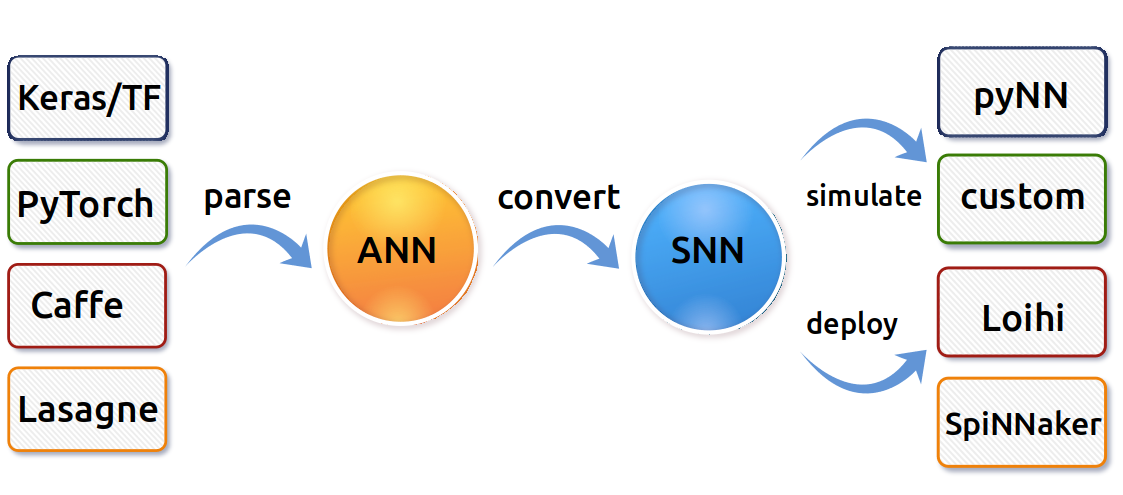
\includegraphics[width=\textwidth]{SNN-TB_workflow}
    \caption{The Illustration of the SNN toolbox workflow. An arbitrary supported deep learning model is transformed to abstract Keras model, which is subsequently converted to spiking network. Source: \url{https://snntoolbox.readthedocs.io/en/latest/guide/intro.html}}
    \label{fig:snn-tb_workflow}
\end{figure}

\section{Keras / Tensorflow}
Keras is a high-level deep learning API which can be used with multiple neural network or machine learning toolkits, mainly with TensorFlow.

\appendix
\chapter{Architecture of the PyNN}
\begin{figure}[htb]
    \centering
    \begin{sideways}
        \includesvg[inkscapelatex=false,width=0.72\textheight]{PyNN_architecture}
    \end{sideways}
    \caption{PyNN architecture}
    \label{fig:pynn_arch}
\end{figure}
\begin{landscape}
    \chapter{State of the community of the spiking simulators}
    \begin{table}[htbp]
        \centering
        \begin{tabularx}{\linewidth}{|>{\raggedright\arraybackslash}X|>{\raggedright\arraybackslash}X|>{\raggedright\arraybackslash}X|>{\raggedright\arraybackslash}X|>{\raggedright\arraybackslash}X|>{\raggedright\arraybackslash}X|>{\raggedright\arraybackslash}X|}
            \hline
            Name & Contributors & mailing list members & GitHub issues & GitHub watchers & License \\                            
            \hline
            \hline
            NEST & 77 & N/A  & 630 & 36 & GPL 2.0 \\
            \hline
            Neuron & 19 & 1516 & 95 & 13 & BSD 3-Clause \\ 
            \hline
            Brian & 27 & 324 & 675 & 42 & custom free software license \\ 
            \hline
            Nengo & 24 & 234 & 730 & 69 & proprietary non-restrictive for non-commercial purposes \\
            \hline
        \end{tabularx}
        \caption{Metrics of the community support for the selected simulation platforms}
        \label{tab:comparison}
    \end{table}
\end{landscape}
\chapter{Evaluation of the documentation of the simulators}
\begin{table}[htbp]
    \centering
    \begin{sideways}
        \begin{tabularx}{0.7\textheight}{*{5}{>{\raggedright\arraybackslash}X}}
            \toprule
             & NEST & Neuron & Brian & Nengo \\
            \midrule
            %     Documentation website & \url{https://nest-simulator.readthedocs.io/} & \url{https://neuron.yale.edu/neuron/docs} & \url{https://brian2.readthedocs.io/} & \url{https://www.nengo.ai/documentation/} \\
            A book describing the simulator & Computational Systems Neurobiology \cite{lenovereComputationalSystemsNeurobiology2012}
            & The NEURON Book \cite{carnevaleNEURONBook06} & & How to build a brain: A neural architecture for biological cognition \cite{eliasmithHowBuild13} \\
            State of the documentation & minor lacks in the Python interface documentation & complete API reference, poorly arranged & minor lacks in API documentation & detailed API reference and tutorials \\
            Is the source code for the tutorials available? & Yes & Yes & Yes & Yes \\
            \bottomrule
        \end{tabularx}
    \end{sideways}
    \caption{Overview of the state of the documentation of the simulators. }
    \label{tab:documentation}
\end{table}
\begin{landscape}
    \chapter{Computation features of the simulators}
    \begin{table}[htbp]
        \centering
        \begin{tabularx}{\linewidth}{|>{\raggedright\arraybackslash}X|>{\raggedright\arraybackslash}X|>{\raggedright\arraybackslash}X|>{\raggedright\arraybackslash}X|>{\raggedright\arraybackslash}X|}
            \hline
                 & NEST & Neuron & Brian & Nengo \\
            \hline
            GPU computation support & No & Yes (coreNEURON library) & Yes (Brian2\-GeNN package) & Yes (OpenCL) \\
            \hline
            parallel computation support & Yes & Yes (special version) & In development (OpenMP) & Yes \\
            \hline
            support for distributed computations & Yes & Yes & No & Yes \\
            \hline
             supported platforms & Linux, MacOS, IBM BlueGene & MS Windows, UNIX, Linux, OS X, IBM Blue Gene, Cray XT3 & Windows, Linux, OS X & Windows, Mac OS X, Linux, Intel Loihi \\
             \hline
        \end{tabularx}
        \caption{Parallelization, high-performance computation support and supported platforms. }
        \label{tab:efficiency}
    \end{table}
\end{landscape}
% 
% PRO ANGLICKOU SAZBU JE NUTNÉ ZMĚNIT
% CITAČNÍ STYL!
%
\emergencystretch=1em

\printbibliography[
heading=bibintoc
]

% \bibliographystyle{ACM-Reference-Format}
% {\raggedright\small
% \bibliography{literature}
% }

\end{document}
